Com a finalidade de validar a interface, foi construído um AV apartir da caracteristicas de um ambiente real(escritório), com planta baixa ilustrada na Figura~\ref{fg:planta_baixa}.\\

 Através de uma antena, foram feitas medições nesse ambiente (sempre mantendo a porta fechada), o que possibilitou a obtenção resposta dele a propagação do sinal dessa antena.\\

\begin{figure}[!htp]
	\centering
	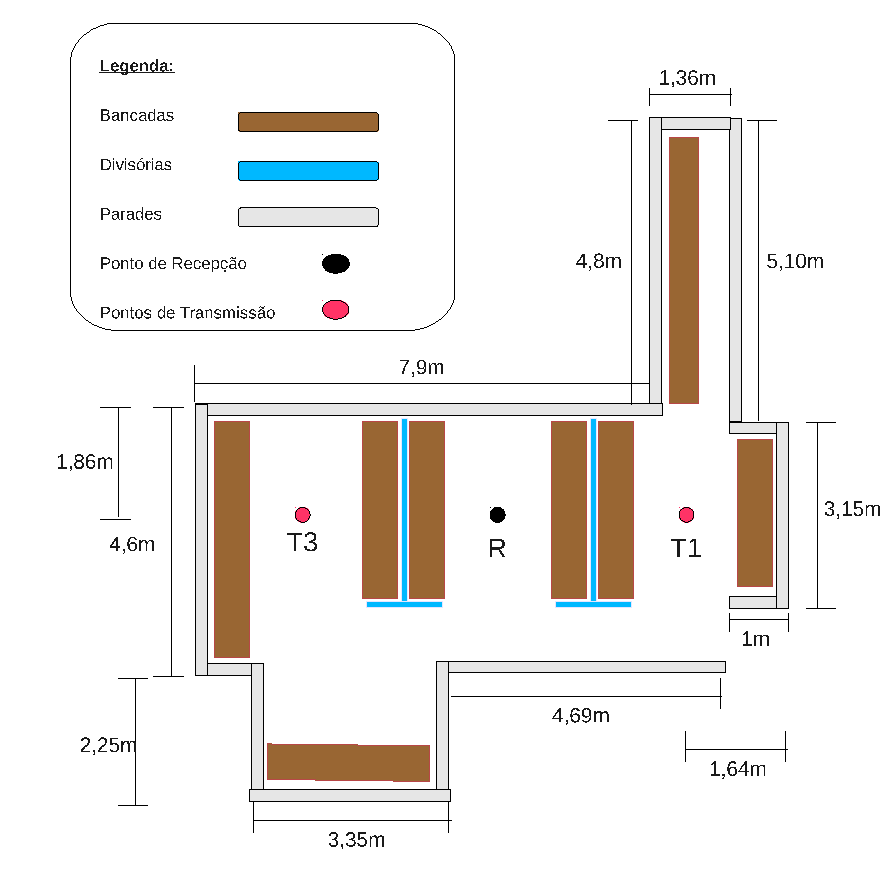
\includegraphics[scale = 1]{planta_baixa}
	\caption{Planta baixa do escritório modelado usando a interface.}
	\label{fg:planta_baixa}
\end{figure}

Todos os objetos presentes na hora das medições foram modelados, sendo eles: computadores, bancadas, monitores, divisórias e paredes divisórias. Suas dimensões estão especificada na Tabela~\ref{tb:objetos}.

\begin{table}
\centering
	\begin{tabular}{|l|l|l|l|}
	\hline
	\textbf{Objetos} & \textbf{Dimensão $X$} & \textbf{Dimensão} $Y$ & \textbf{Dimensão $Z$}\\ \hline
	Computadores (CPU's) & $0,18m$ & $0,43m$ & $0,42m$ \\ \hline
	Monitores & $0,39m$ & $0,31m$ & $0,39m$ \\ \hline
	Divisórias $1$ e $2$ & $3,27m$ & $1,5m$ & $0,03m$ \\ \hline
	Paredes divisórias $1$ e $2$ & $0,03m$ & $1,5m$ & $1m$ \\ \hline
	Bancadas de $1$-$4$ & $3,21m$ & $0,03m$ & $0,5m$ \\ \hline
	Bancada $5$ & $2,94m$ & $0,03m$ & $0,5m$ \\ \hline
	Bancada $6$ & $4,68m$ & $0,03m$ & $0,5m$ \\ \hline
	Bancada $7$ & $0,5m$ & $0,03m$ & $3,18m$ \\ \hline
	Bancada $8$ & $4,26m$ & $0,03m$ & $0,5m$ \\
	\hline
	\end{tabular}
	\caption{Objetos e suas dimensões.}
	\label{tb:objetos}
\end{table}

Alguns desse objetos estão dispostos em alturas diferentes em relação ao piso. As bancadas e o teto estão a uma altura de 0,75 metros e 2,73 metros, respectivamente. Os computadores e monitores foram colocados uma célula acima do nível das bancadas, como a altura das bancadas é de 25 células, eles foram modelados apartir da célula 26 (equivalente a uma altura de 0,78m).\\

As dimensões gerais desse cenário usadas na interface, foram:
\begin{itemize}
\item \textit{Delta}(Tamanho da célula de Yee) utilizada foi de $0,003m$.
\item \textit{Região de Análise} com dimensões: $X$ = $15m$, $Y$ = $3m$ e $Z$ = $15m$.
\item \textit A lista das carateristicas físicas com seus respectivos matérias estam presentes na Tabela~\ref{tab:materiais}
\end{itemize}

\begin{table}
\centering
	\begin{tabular}{|l|l|l|l|l|}
	\hline
	Elementos dos Ambiente & Material & $\epsilon$ & $\sigma$ & $\mu$ \\ \hline
	Parede & Tijolo & $4$ & $0,0135$ & $1$\\ \hline
	Teto & Gesso & $2,8$ & 0,1533 & 1 \\ \hline
	Bancadas & Madeira & $1,8$ & $0,011$ & $1$\\ \hline
	Monitores e Gabinetes & Metal & $5$ & $1\times10^{11}$ & $1$\\ \hline
	Divisórias & Vidro & $5$ & $5\times10^{-4}$ & $1$ \\ \hline
	Piso & Concreto & $5$ & $1$ & $1$ \\
	\hline
	\end{tabular}
	\caption{Tabela de elemetos, materiais parâmetros físicos.}
	\label{tab:materiais}
\end{table}

Como resultado da modelagem usando a interface, obeteve-se as estruturas mostradas nas Figuras~\ref{fg:ambiente} e \ref{fg:amb_sags} . A disposição dos seus objetos tentou seguir o posicionamento real dos mesmos no momento das medições.

\begin{figure}[!tp]
	\centering
	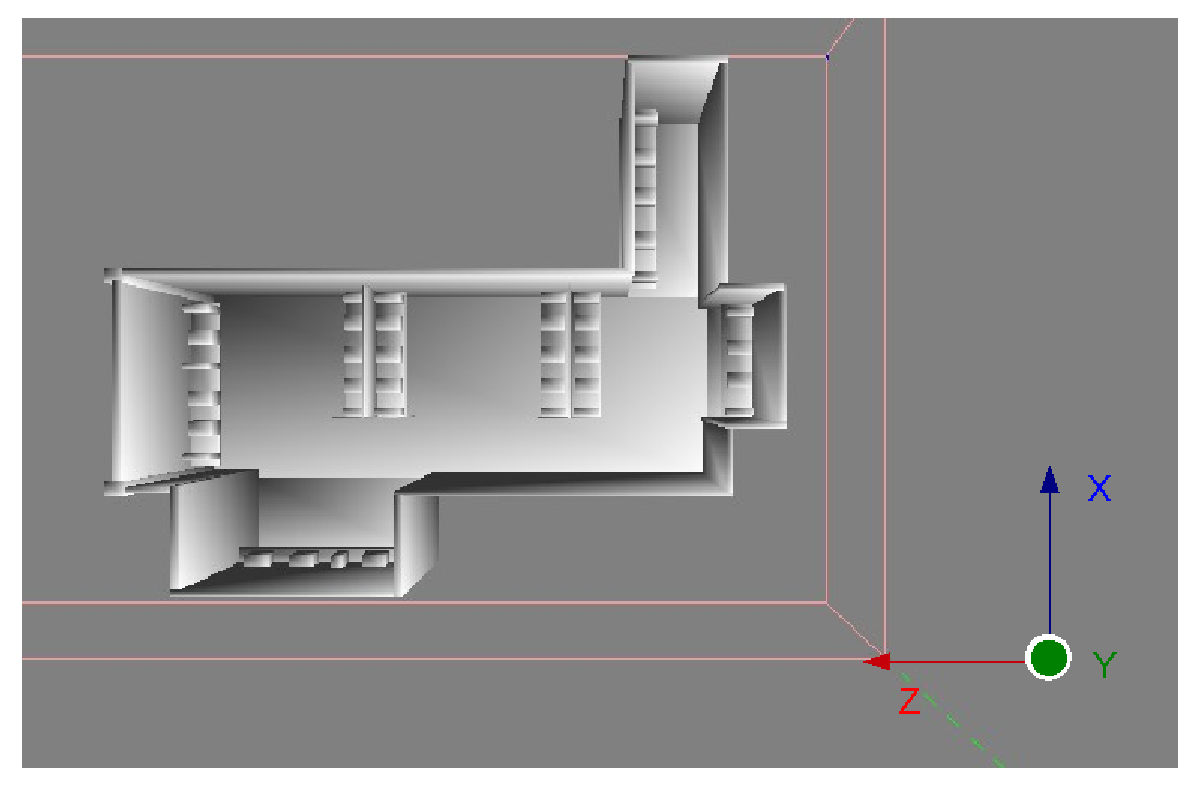
\includegraphics[scale = 0.4]{ambiente}
	\caption{Visão topo em pespectiva do ambiente construído na interface.}
	\label{fg:ambiente}
\end{figure}
\begin{figure}[!tp]
	\centering
	\includegraphics[scale = 0.4]{amb_sags}
	\caption{Visão em pespectiva do cenário no simulador LANE-SAGS.}
	\label{fg:amb_sags}
\end{figure}

%antenas e fontes
Depois de ambiente ter sido montado, surguiu a necessidade de introduzir a antena. Como a que foi usada na medição tinha uma forma complicada para modelagem, foi necessário criar uma que além de representar, funcionasse de forma semelhante com a real. Após fazer uma análise, percebeu-se que a antena usada  durante as medições funcionava como um dipolo. Assim, alguns testes foram realizados desejando encontrar uma representação aceitável para o problema.\\

Para todos os modelos de antenas criados, foi ultizada uma fonte de tensão de trêm de pulsos normalizado(Equação~\ref{eq:trem}), Figura~\ref{fg:tensao}, onde através da transforma de Fourier, pode-se observar se a mesma estava trabalhando na banda adequada (a banda de trabalho da antena real é de $700MHz$-$900MHz$). O resultado obtido foi o ilustrado na Figura~\ref{fg:f_fonte}.\\

\begin{equation}\label{eq:trem}
	P(f) = A_p\exp~\big(-{\frac{t-3T}{T}}^{2}\big)\exp(\frac{t-3T}{T})
\end{equation}
Onde:\\
$A_p = 1$ e $T$ =  $6.53846\times10^{-10}$
\begin{figure}[!ht]
	\begin{center}
		\subfigure[Gráfico da fonte(trem de pulsos) no tempo.]{\label{fg:tensao}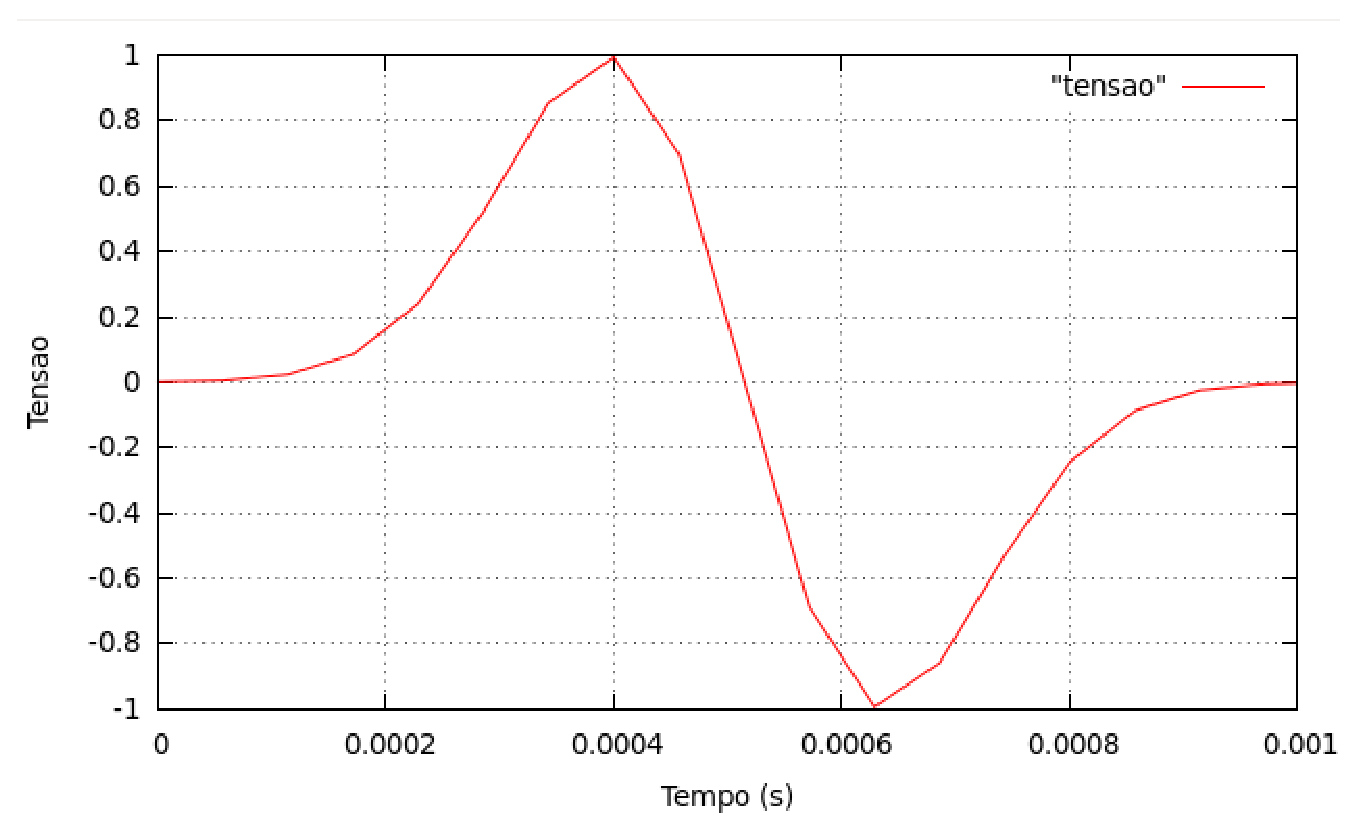
\includegraphics[scale=0.3]{tensao}}
\qquad
		\subfigure[Gráfico da transformada de Fourier da fonte.]{\label{fg:f_fonte}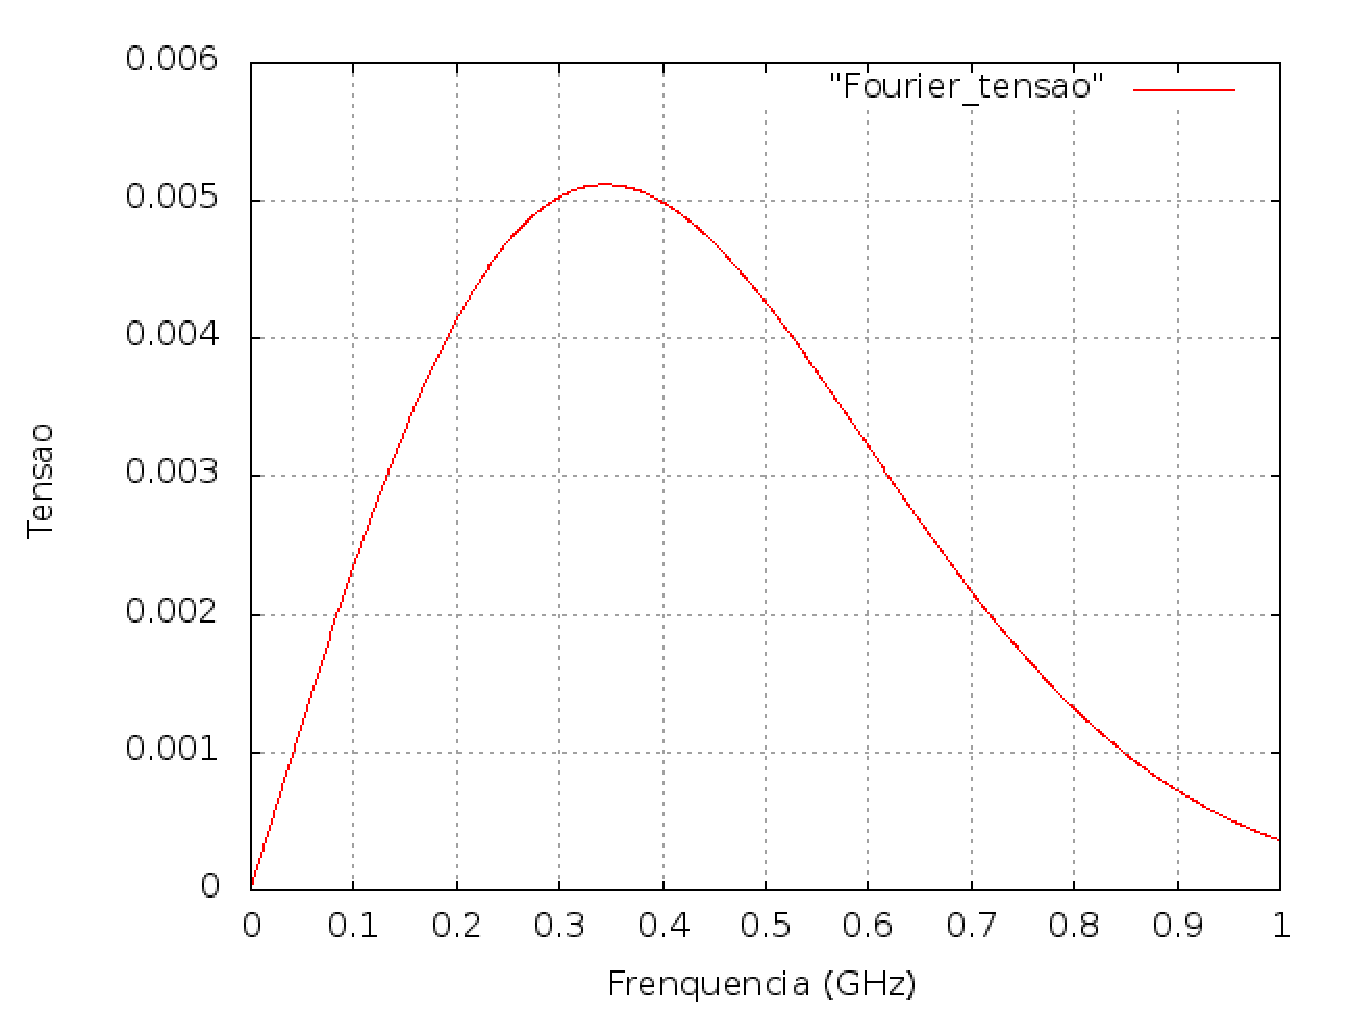
\includegraphics[scale=0.3]{f_fonte}}
	\end{center}
	\caption{Fonte de tensão usada nas antenas modeladas.}
	\label{fg:fontes}
\end{figure}

A primeira antena teste feita foi a mostrada no diagrama da Figura~\ref{fg:antena_normal}, juntamente com sua representação no LANE-SAGS(Figura~\ref{fg:antena_normal_sags}). Os blocos do seu diagrama tem as mesmas dimensões, assim como as hastes. Ela foi testada colocando a fonte entre as hastes, medindo a corrente nas extremidades da haste a esquerda e a tensão na mesma posição da fonte. \\

\begin{figure}[!ht]
	\begin{center}
		\subfigure[Diagrama da primeira antena dipolo criada.]{\label{fg:antena_normal}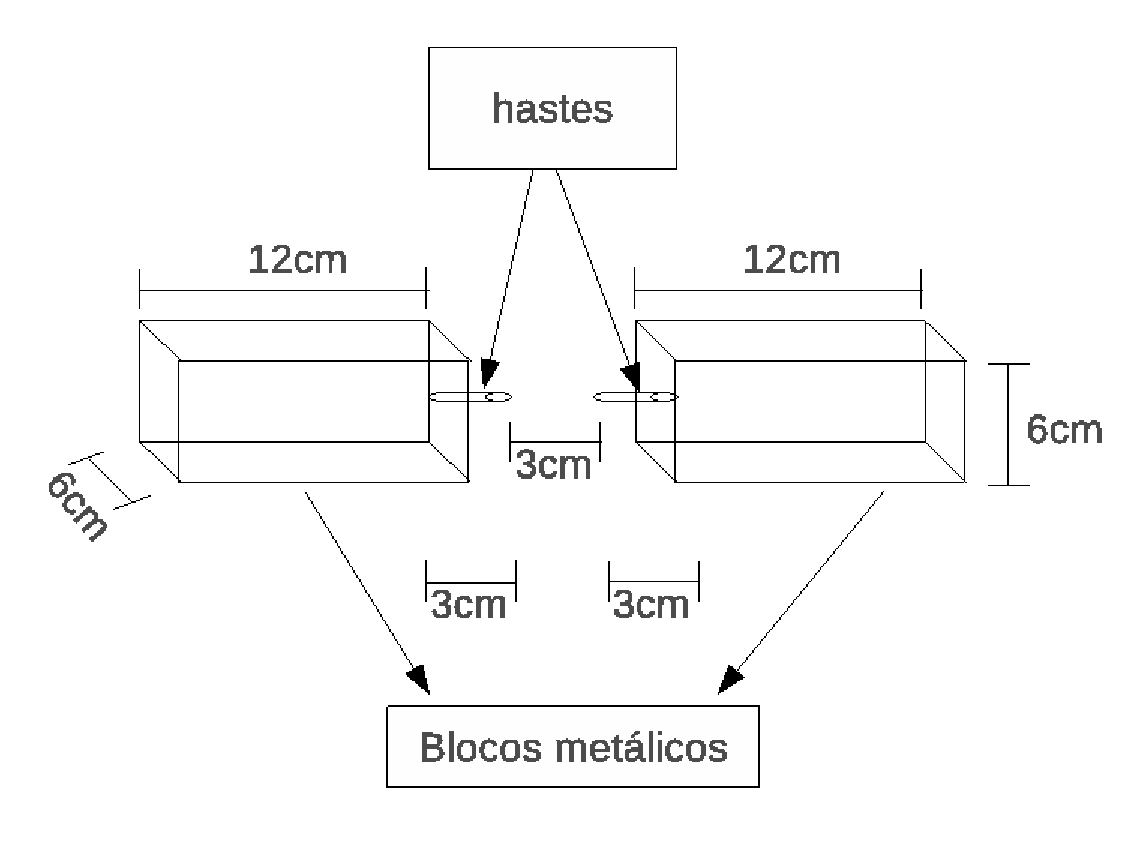
\includegraphics[scale=0.25]{antena_normal}}
\qquad
		\subfigure[Visualização da primeira antena no simulador LANE-SAGS.]{\label{fg:antena_normal_sags}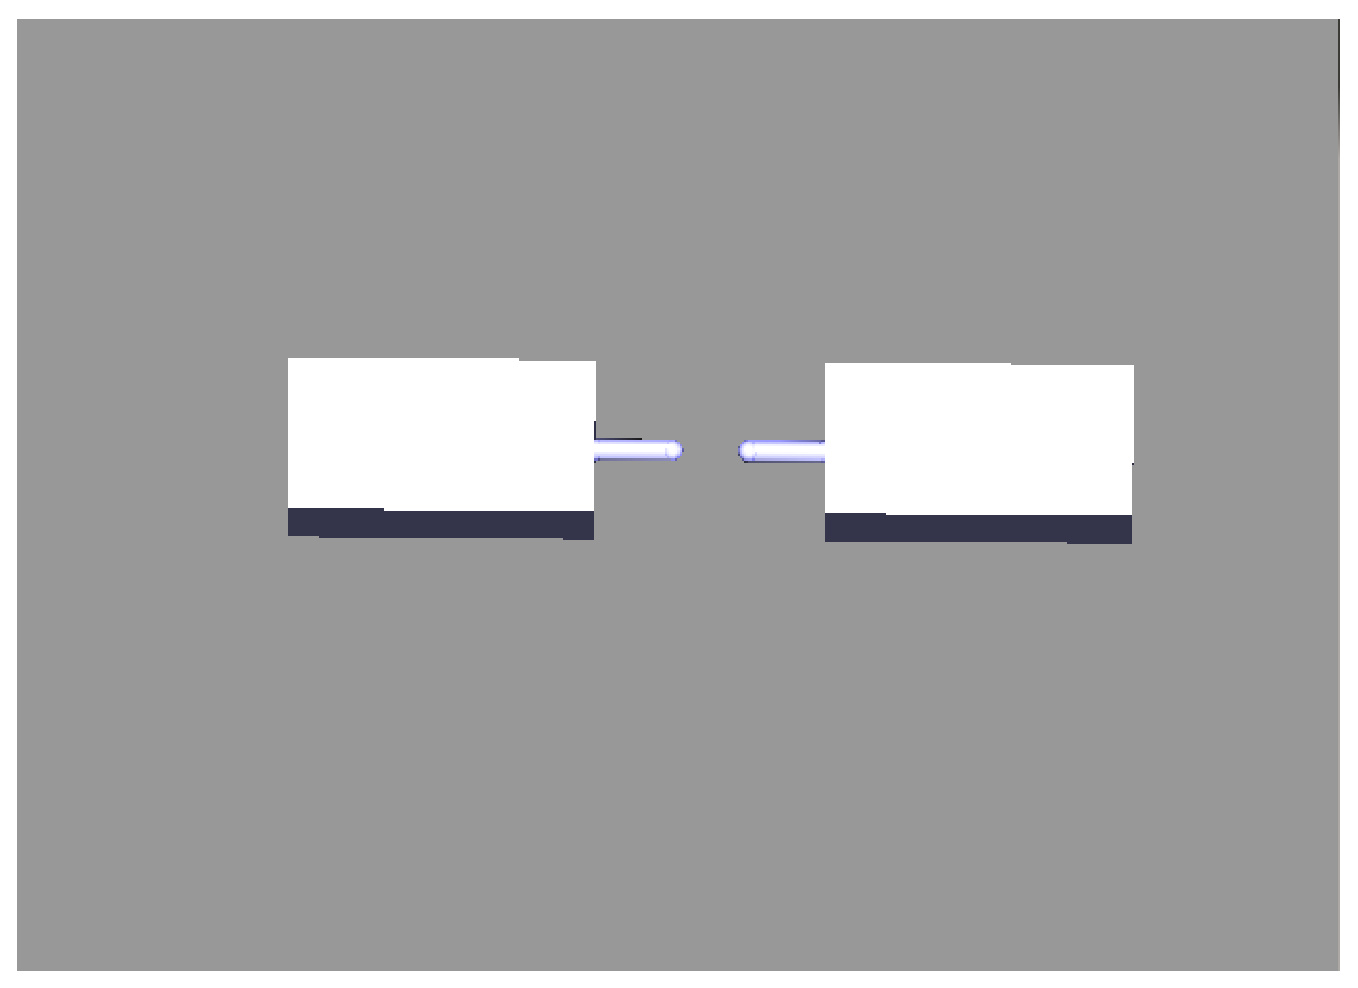
\includegraphics[scale=0.25]{antena_normal_sags}}
	\end{center}
	\caption{Antena dipolo normal.}
	\label{fg:antena_normal_m}
\end{figure}

Com os dados de tensão e corrente, foi calculado o coeficiente de reflexão dessa antena através da fórmula mostrada na Equação~\ref{eq:impedancia}. Por meio dele pode-se computar a perda de retorno, Figura~\ref{fg:pr_01}, associada a essa antena(Equação~\ref{eq:pr}). Como pode-se observar na figura, a antena esta trabalhando abaixo de $-10dB$ em uma faixa diferente da desejada($700MHz-900MHz$). Portanto, suas dimensões e parâmentros necessitaram ser modificados.\\

\begin{figure}[!ht]
	\centering
	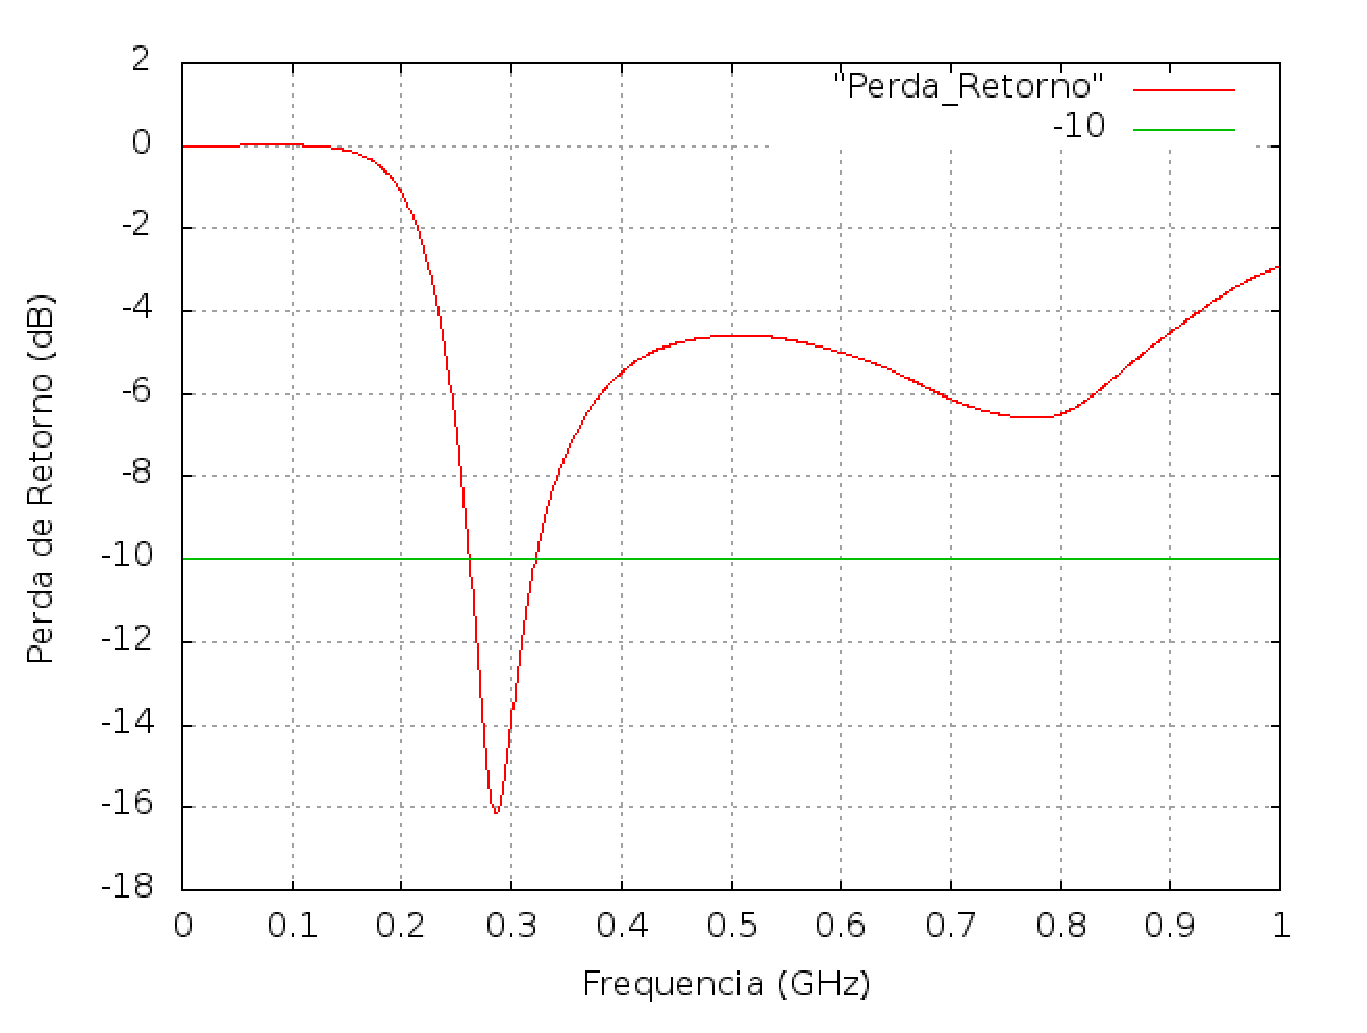
\includegraphics[scale = 0.5]{pr_01}
	\caption{Perda de retorno da antena dipolo normal(primeira antena modelada).}
	\label{fg:pr_01}
\end{figure}

\begin{equation}\label{eq:impedancia}
	\Gamma = \frac{Z_{L} - Z_{S}}{Z_{L} + Z_{S}}
\end{equation}
Onde: $Z_{S}$ é a impedãncia de entrada($50 ohm$) e $Z_{L}$ representa a impedância relacionada a carga(calculada ponto a ponto com dados de tensão pela corrente coletados).
\begin{equation}\label{eq:pr}
	RL(dB) = -20log_{10} |\Gamma|
\end{equation}

Após alguns teste, verificou-se que a diminuição na dimensão dessa antena afetava de forma positiva o resultado da perda de retorno, porém tinhamos um impasse ligado ao fato do tamanho do \textit{delta}(que diminuiria de forma proporcional). Portanto se a diminuiçao fosse grande, ficaria improvavel a simulação desse ambiente, mesmo ele sendo pequeno, pelo seu custo computacional. Surgiu então a idéia do uso de um capacitor(com capacitância igual a $3,7\times10^{-5} farad$) aclopado um dos blocos métalicos, através de sua impedância simularia a diminuição sem precisarmos de fato mexer tanto nas dimensões da antena.\\

A configuração da antena adaptada esta ilustrada no diagrama da Figura~\ref{fg:antena_final}. A Figura~\ref{fg:antena_final_sags} mostra ela no LANE-SAGS. Os cálculos feitos para antena anterior foram refeitos, como resultado obteve-se a perda de retorno desejada mostrada na Figura~\ref{fg:pr_2}, que faz também uma comparação com a obtida anteriormente.\\

\begin{figure}[!ht]
	\centering
	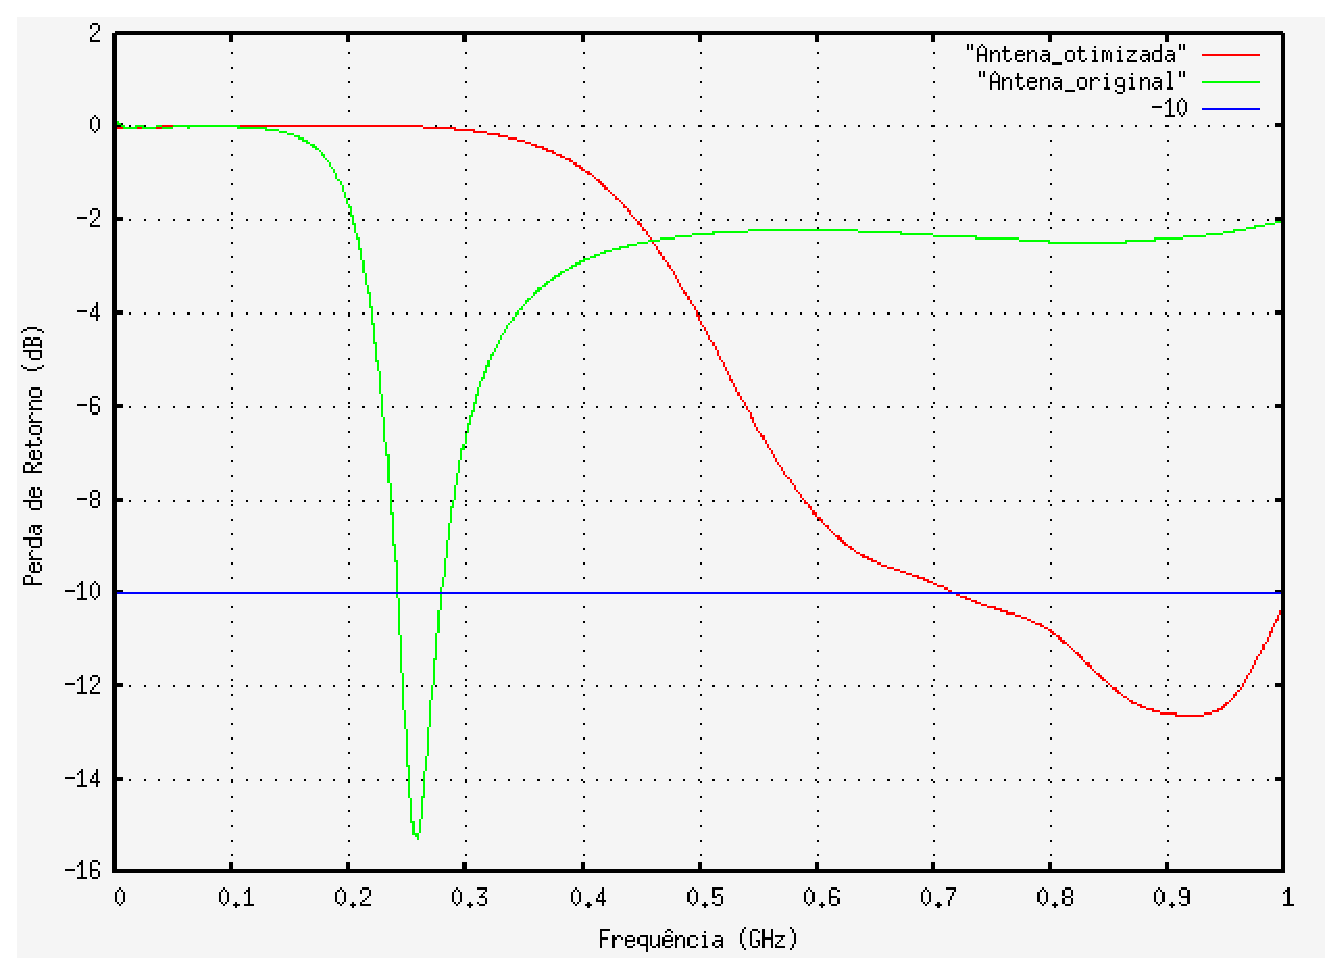
\includegraphics[scale = 0.5]{pr_2}
	\caption{Comparação entre as perdas de retorno da antena otimizada(adaptada) e normal(original).}
	\label{fg:pr_2}
\end{figure}

\begin{figure}[!ht]
	\begin{center}
		\subfigure[Diagrama da antena dipolo adaptada.]{\label{fg:antena_final}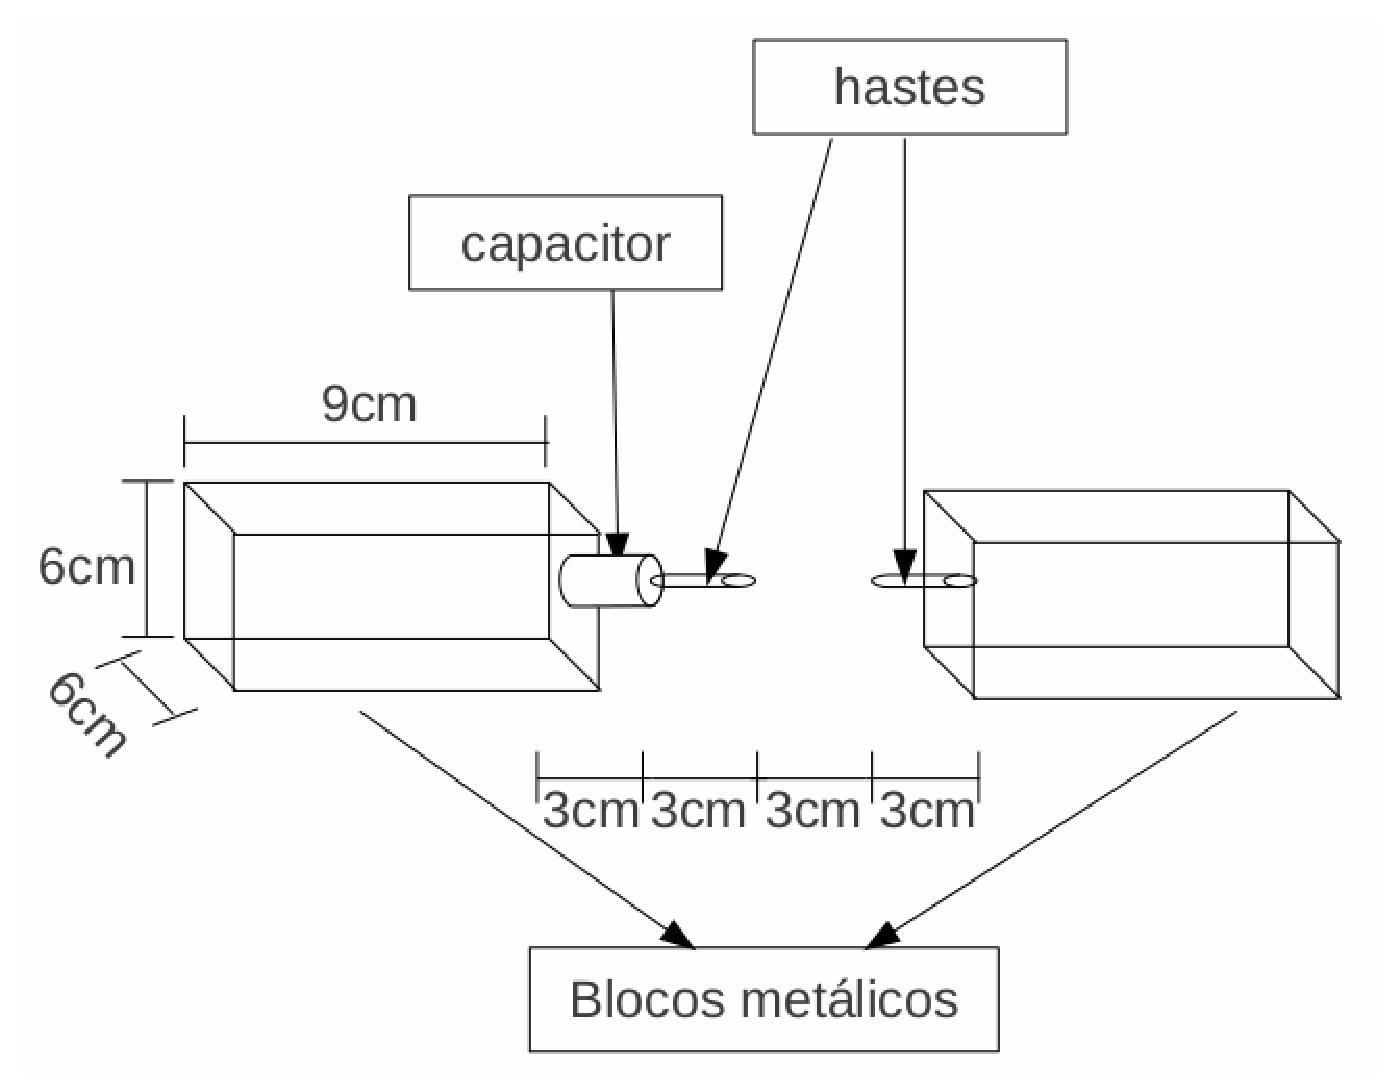
\includegraphics[scale=0.25]{antena_final}}
\qquad
		\subfigure[Visualização da antena adaptada no simulador LANE-SAGS.]{\label{fg:antena_final_sags}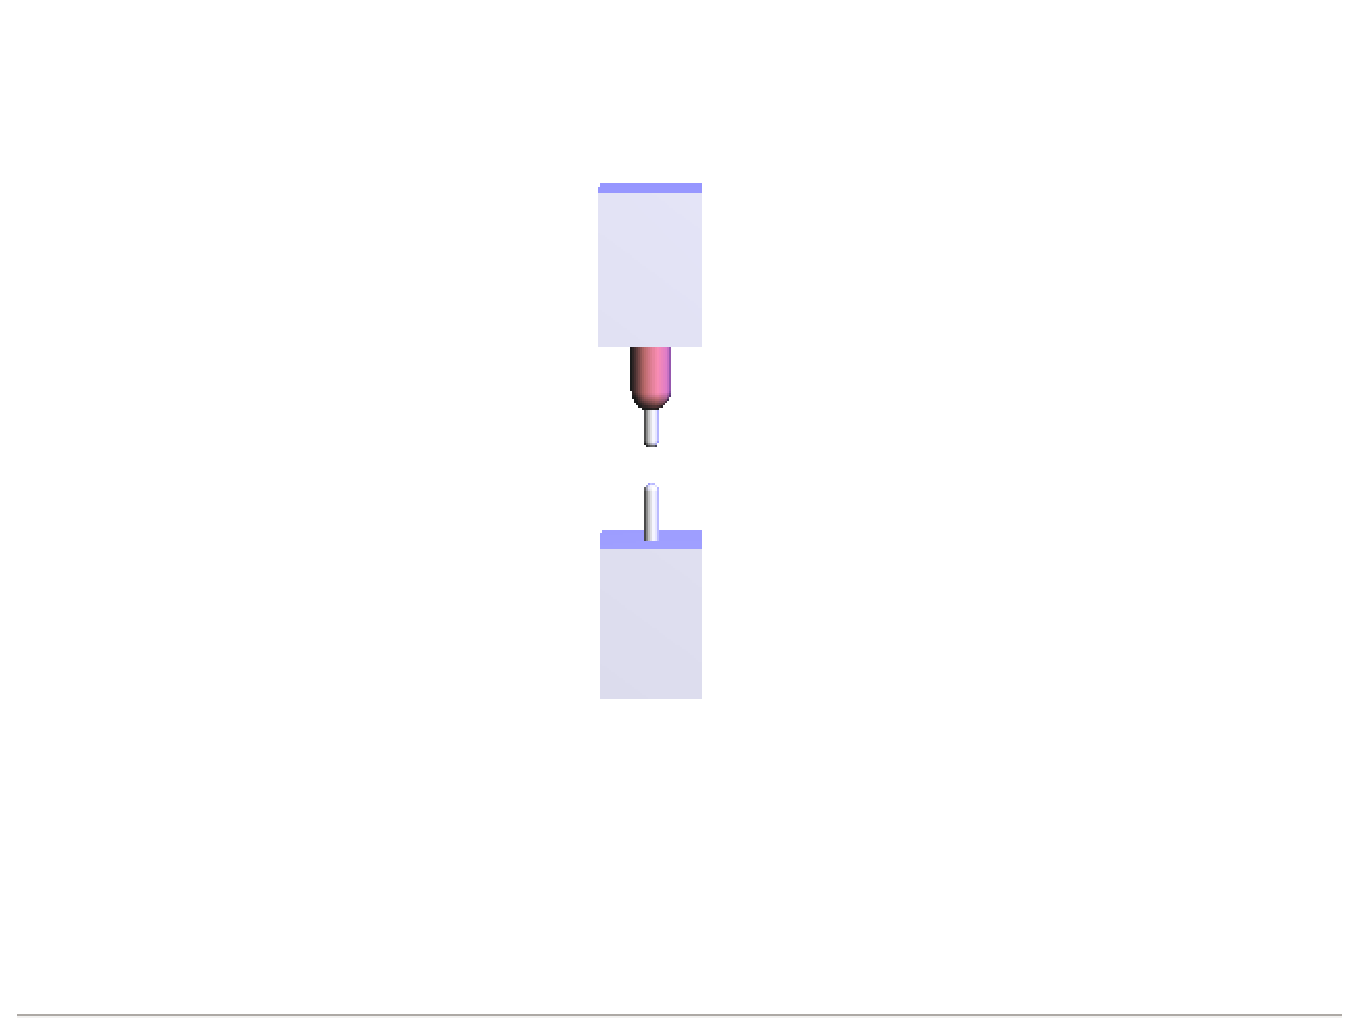
\includegraphics[scale=0.25]{antena_final_sags}}
	\end{center}
	\caption{Antena dipolo adaptada.}
	\label{fg:antena_apatada}
\end{figure}

%resultados
\subsection{Caso 01}
O caso 01 refere-se a introdução da antena modelada na posição $T1$ da Figura~\ref{fg:planta_baixa}. Ela foi posicionada a uma altura de $1,5m$ do piso. Com isso foi feita a simulação obteve-se além da tensão calculada no ponto R(que tem a mesma altura do ponto $T1$) do cenário modelado, a tensão entre as hastes da antena. Esse sinais estão mostrados nas Figuras~\ref{fg:t_out} e \ref{fg:t_in}.

\begin{figure}[!ht]
	\begin{center}
		\subfigure[Gráfico da tensão no Ponto R.]{\label{fg:t_out}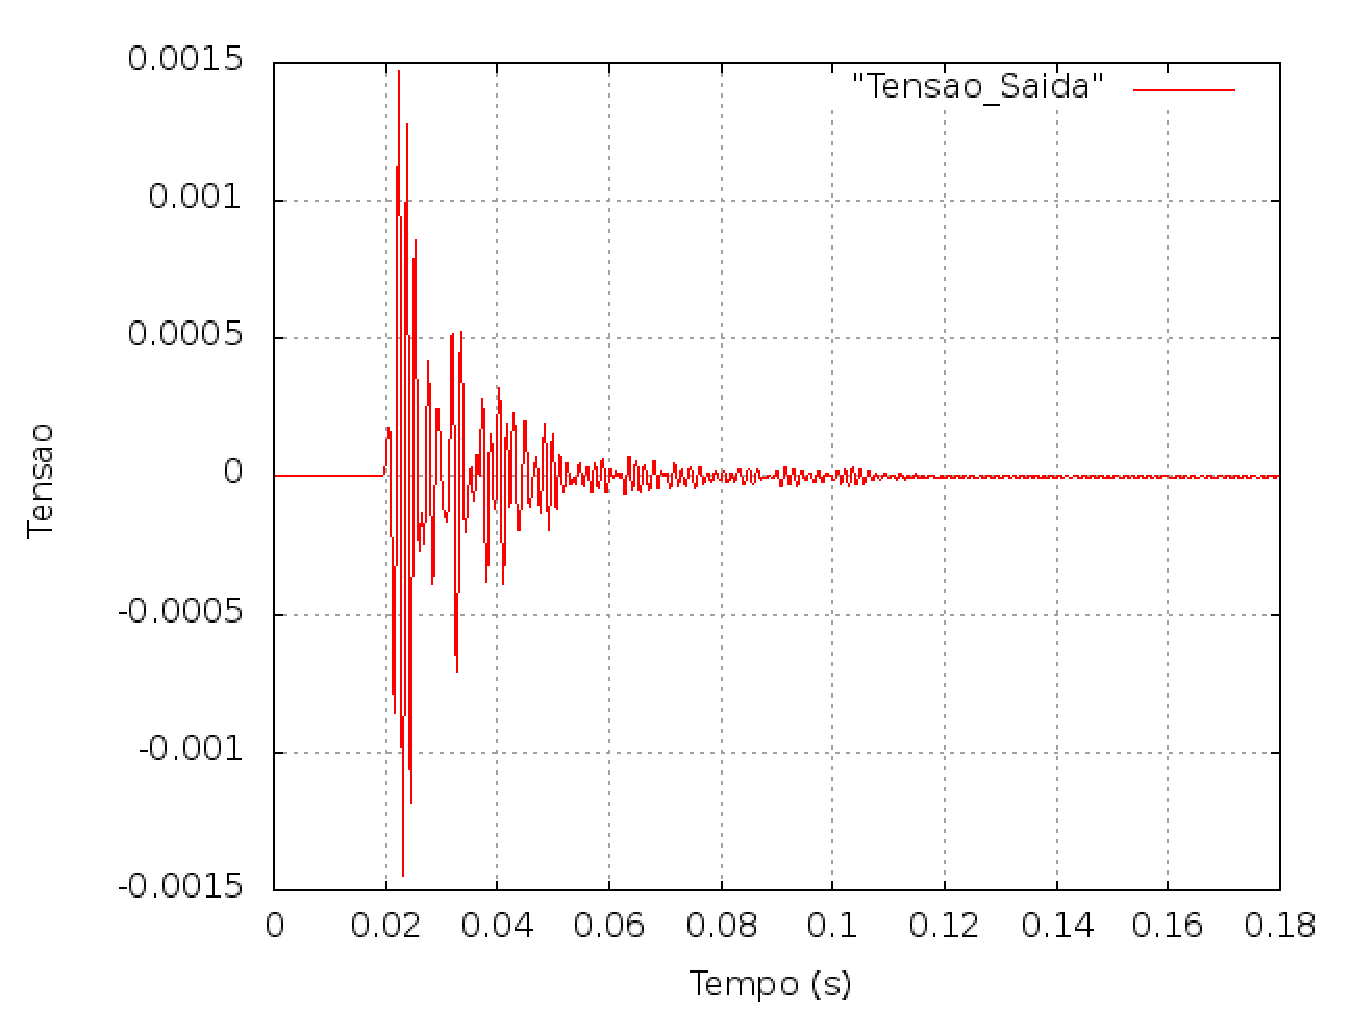
\includegraphics[scale=0.25]{t_out}}
\qquad
		\subfigure[Gráfico da tensão no Ponto $T1$(entre as hastes da antena).]{\label{fg:t_in}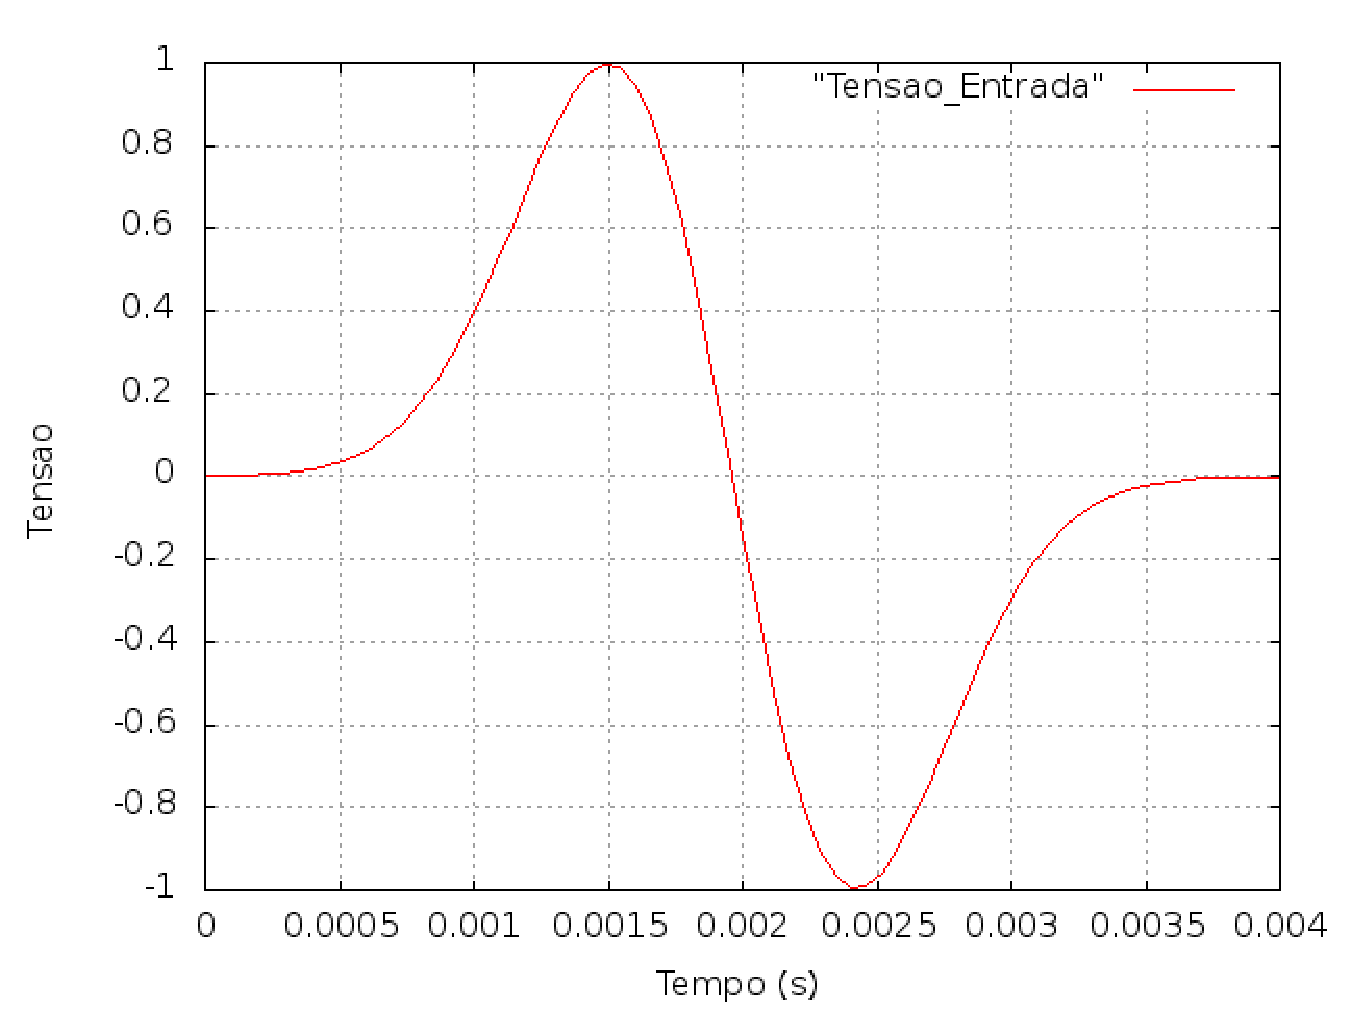
\includegraphics[scale=0.25]{t_in}}
	\end{center}
	\caption{Tensões obtidas pela simulação.}
	\label{fg:tensoes}
\end{figure}

Por meio desses dados de entrada e saída, desejava-se calcular o perfil de potência e retardo do canal, Equação~\ref{eq:potencia}, desse ambiente virtual simulado, para comparar com o medido. Todavia, para que isso fosse possível, era necessário ter a resposta impulsiva desse canal. A Figura~\ref{fg:hf} mostra o processo de obtenção da resposta em frequência.\\

\begin{equation}\label{eq:potencia}
	P_h(\tau) = |h(\tau)|^{2}
\end{equation}
\begin{figure}[!ht]
	\centering
	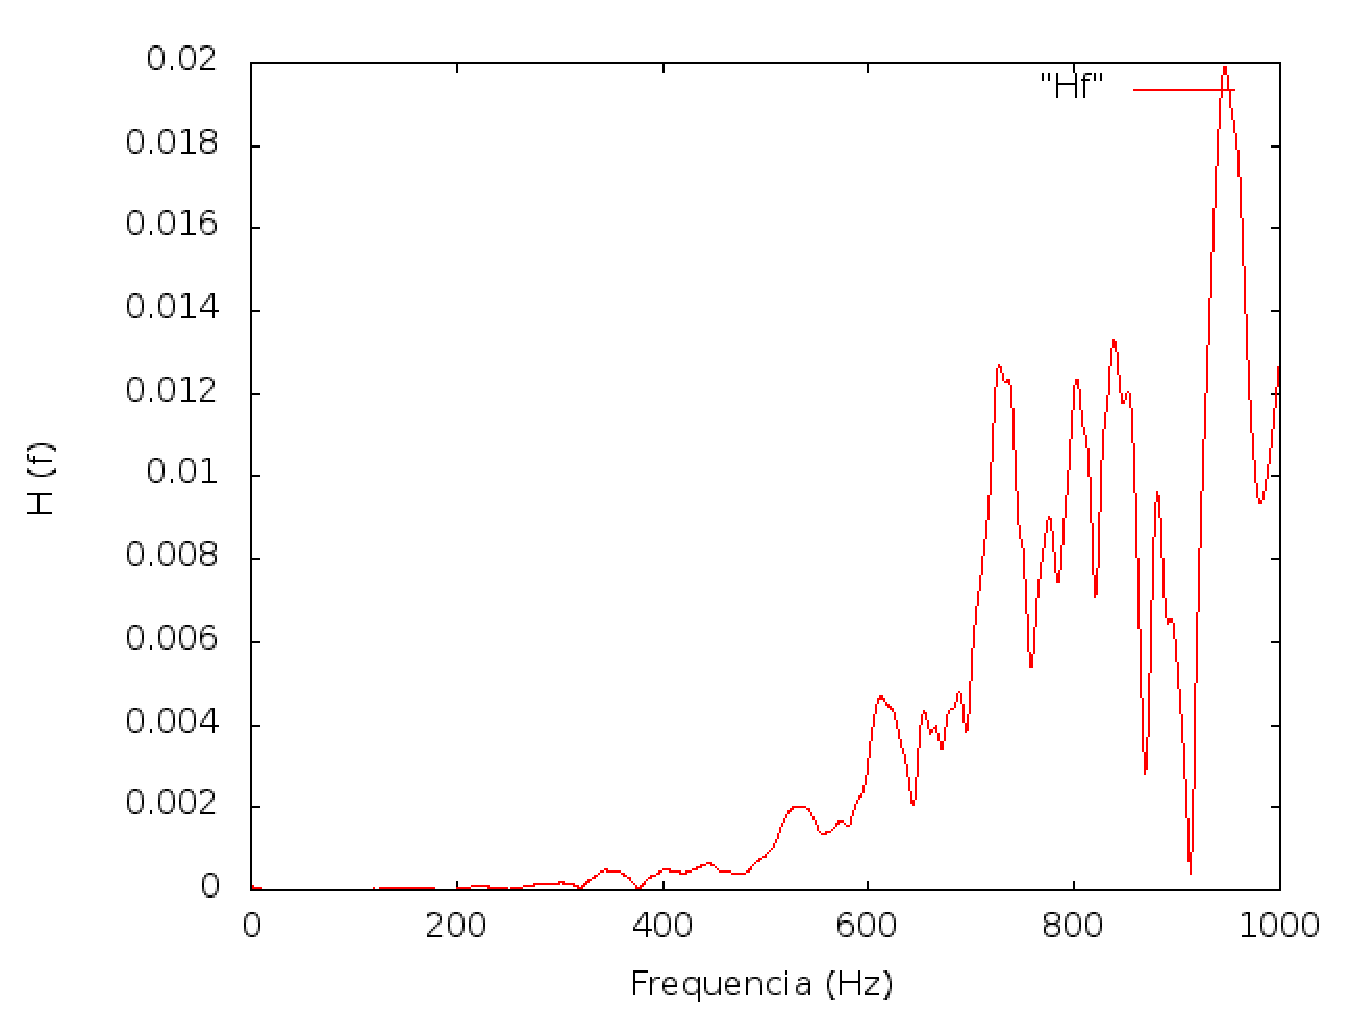
\includegraphics[scale = 0.5]{hf}
	\caption{Diagrama de bloco ilustrando a operação linear de obtenção da função de transferência $H(f)$.}
	\label{fg:hf}
\end{figure}

Logo, as tensões de entrada(referente ao ponto $T1$) e saída (referente ao ponto $R$), usando a transformada de Fourier, foram lanchadas para o domínio da frequência e então divididas ponto a ponto. Com isso se obteve a resposta em frequência, $H( f )$. Usando a Equação~\ref{eq:ant_f},referente a anti transformada de Fourier, se obter a resposta impulsiva desse canal.\\


Usando a Equação~\ref{eq:ant_f} foi possível obter a função de transferência no domínio do tempo e assim comparar o perfil de potência e retardo obtido pela simulação com o medido. A Figura~\ref{fg:ms} mostra essa comparação.

\begin{equation}\label{eq:ant_f}
	h(\tau) = \mathcal{F}^{-1}{H(f)}
\end{equation}

\begin{figure}[!ht]
	\centering
	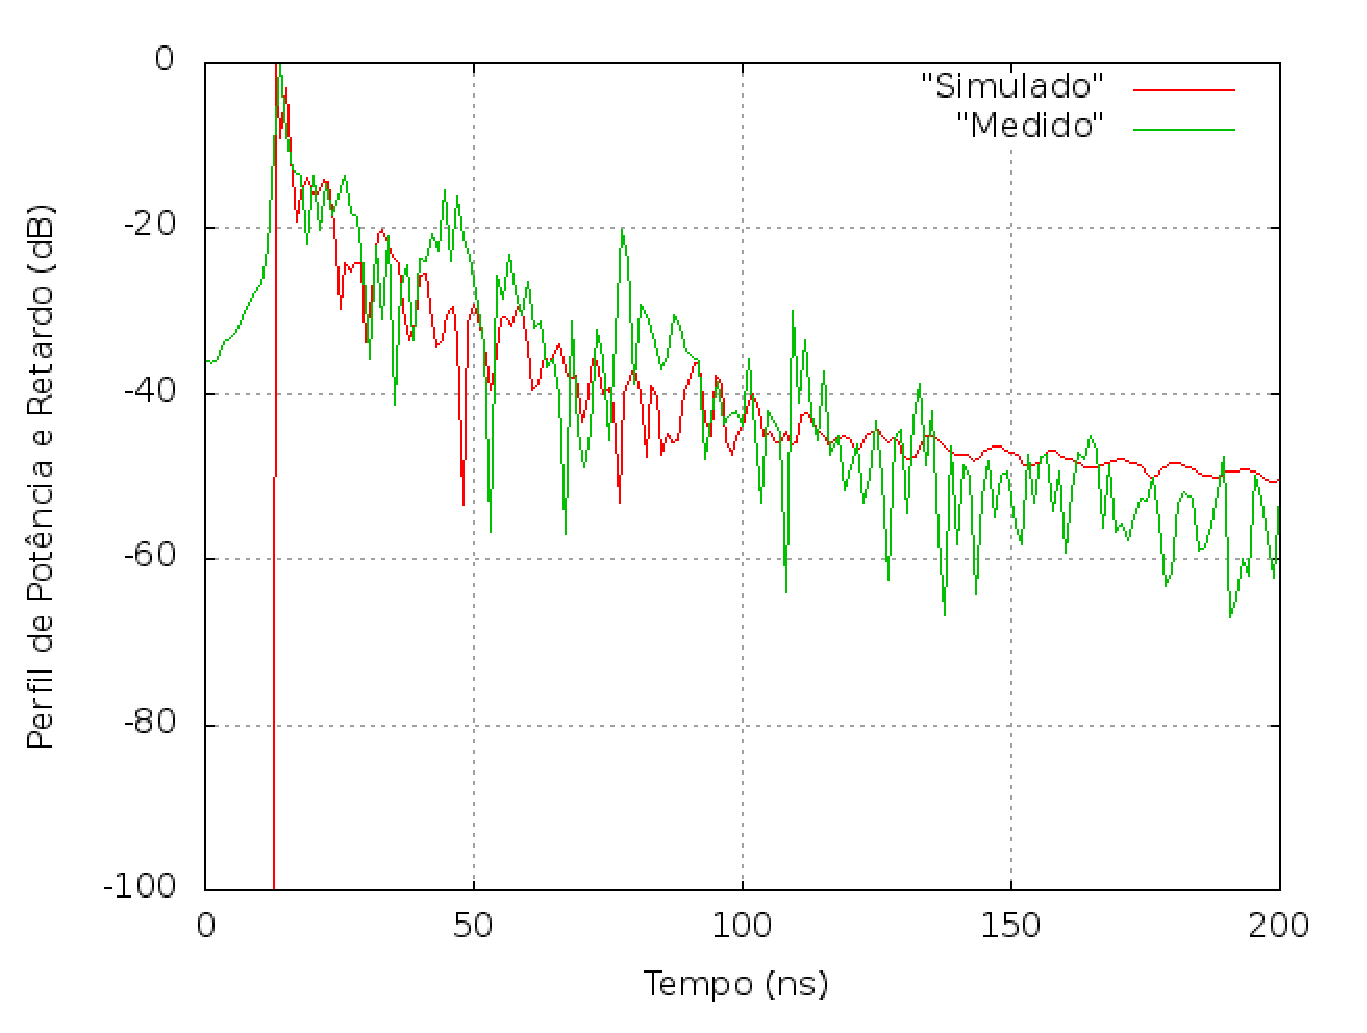
\includegraphics[scale = 0.5]{ms}
	\caption{Comparação entre medição e simulação.}
	\label{fg:ms}
\end{figure}
